\lstinputlisting[language=Python]{../assignment_c1.py}
\pagebreak

\section*{BONUS til oppgave 1b \& c:}
For $y^*$ kan jeg velge å skalere med toppunktet til $y(t)$.
Det finner vi ved å sette inn en halv $t_m$ (fordi dette er en parabel
og toppunktet halvveis mellom to ekvivalente verdier, altså $t = 0$ og $t_m$):

\begin{align*}
    &y(t) = v_0t \sin{\theta} - \frac{1}{2}gt^2
    \\
    &y(0.5t_m) = v_0\frac{v_0}{g}\sin{\theta} \sin{\theta}
    - \frac{1}{2}g\frac{v_0^2}{g^2}\sin^2{\theta}
    \\
    &y(0.5t_m) = \frac{v_0^2}{g}\sin^2{\theta}
    - \frac{1}{2}\frac{v_0^2}{g}\sin^2{\theta}
    \\
    &y(0.5t_m) = \frac{1}{2}\frac{v_0^2}{g}\sin^2{\theta}
\end{align*}

Dermed blir den dimensjonsløse variabelen for y:

\begin{align*}
    y^* = y/y(0.5t_m)
\end{align*}

\begin{figure}[H]
		\centering
		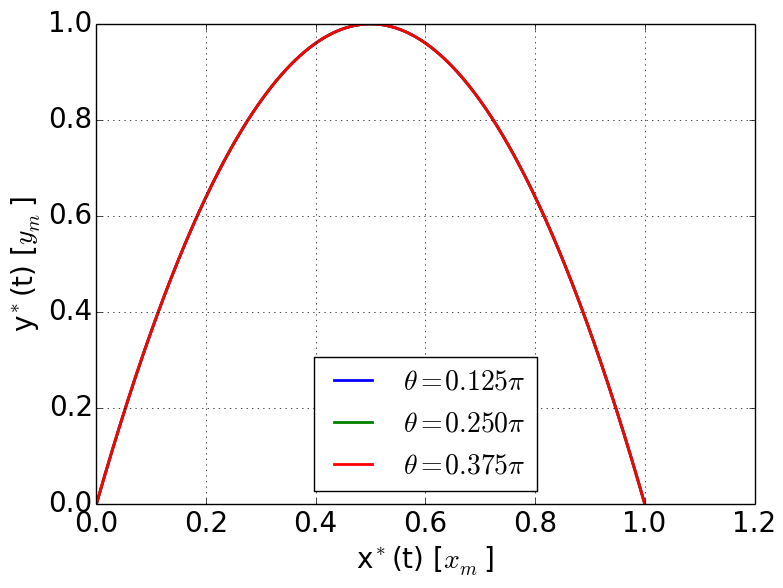
\includegraphics[width=0.7\linewidth]{../alternativ_skalering.png}
		\caption{Grafen viser hvordan banene til ballene med forskjellige
        utkastvinkel vil være i xy-planet. Programmet som ble brukt for
        å lage denne figuren finner du bakerst i innleveringen.}
		\label{fig_alternativ}
\end{figure}

Denne innføringen av dimensjonsløse variabler, gjør at alle kast ser like ut.
Det er en vis sannhet i det (de uttrykkes ved samme formel). Skaleringen gjør
at informasjonen om vinkelen også er pakket inn i aksene, som beskrevet i 1 c).
\pagebreak

\begin{figure}[H]
		\centering
		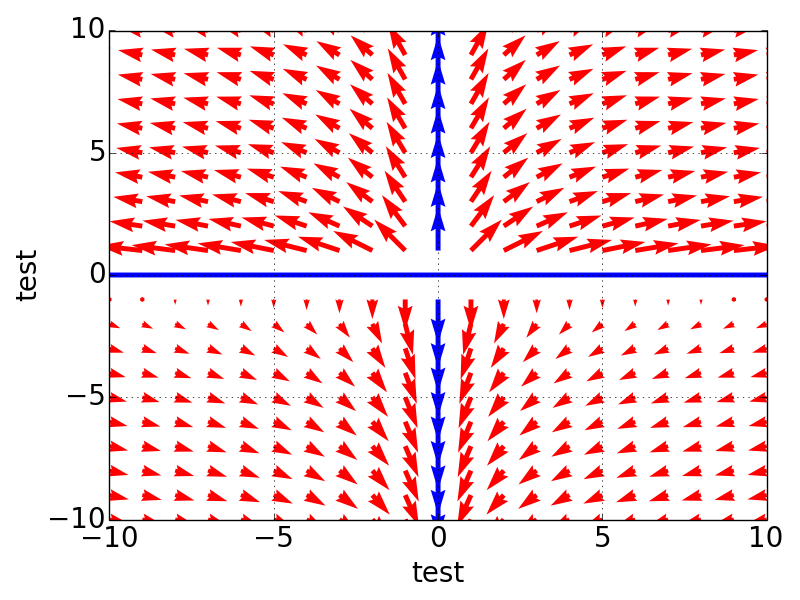
\includegraphics[width=0.7\linewidth]{../test.png}
		\caption{Dette er et tidligere forsøk på å vise
         strømvektorene til 2 b). Fargene er for å gjenskape vårt
         fantastiske flag :).}
		\label{fig_2b_test}
\end{figure}

\pagebreak


\pagebreak
\lstinputlisting[language=Python]{../assignment_b2.py}
\pagebreak
\lstinputlisting[language=Python]{../assignment_b3.py}
\pagebreak

\lstinputlisting[language=Python]{../streamfun.py}
\lstinputlisting[language=Python]{../strlin.py}

\pagebreak
\lstinputlisting[language=Python]{../velfield.py}
\lstinputlisting[language=Python]{../vec.py}


















%
